\documentclass{article} % For LaTeX2e
\usepackage{nips14submit_e,times}
\usepackage{amsmath}
\usepackage{amsthm}
\usepackage{amssymb}
\usepackage{mathtools}
\usepackage{hyperref}
\usepackage{url}
\usepackage{algorithm}
\usepackage[noend]{algpseudocode}
%\documentstyle[nips14submit_09,times,art10]{article} % For LaTeX 2.09

\usepackage{mathrsfs}
\usepackage{graphicx}
\usepackage{caption}
\usepackage{subcaption}

\def\eQb#1\eQe{\begin{eqnarray*}#1\end{eqnarray*}}
\def\aB#1\aE{\begin{align*}#1\end{align*}}
\def\eQnb#1\eQne{\begin{align}#1\end{align}}
\providecommand{\e}[1]{\ensuremath{\times 10^{#1}}}
\providecommand{\pb}[0]{\pagebreak}

\newcommand{\E}{\mathrm{E}}
\newcommand{\Var}{\mathrm{Var}}
\newcommand{\Cov}{\mathrm{Cov}}

\def\Qb#1\Qe{\begin{question}#1\end{question}}
\def\Sb#1\Se{\begin{solution}#1\end{solution}}

\usepackage{scalerel,stackengine}
\stackMath
\newcommand\reallywidehat[1]{%
\savestack{\tmpbox}{\stretchto{%
  \scaleto{%
    \scalerel*[\widthof{\ensuremath{#1}}]{\kern-.6pt\bigwedge\kern-.6pt}%
    {\rule[-\textheight/2]{1ex}{\textheight}}%WIDTH-LIMITED BIG WEDGE
  }{\textheight}% 
}{0.5ex}}%
\stackon[1pt]{#1}{\tmpbox}%
}

\newenvironment{claim}[1]{\par\noindent\underline{Claim:}\space#1}{}
\newtheoremstyle{quest}{\topsep}{\topsep}{}{}{\bfseries}{}{ }{\thmname{#1}\thmnote{ #3}.}
\theoremstyle{quest}
\newtheorem*{definition}{Definition}
\newtheorem*{theorem}{Theorem}
\newtheorem*{lemma}{Lemma}
\newtheorem*{question}{Question}
\newtheorem*{preposition}{Preposition}
\newtheorem*{exercise}{Exercise}
\newtheorem*{challengeproblem}{Challenge Problem}
\newtheorem*{solution}{Solution}
\newtheorem*{remark}{Remark}
\usepackage{verbatimbox}
\usepackage{listings}
\title{Harmonic Analysis:  \\
Final Exam}


\author{
Youngduck Choi \\
CIMS \\
New York University\\
\texttt{yc1104@nyu.edu} \\
}


% The \author macro works with any number of authors. There are two commands
% used to separate the names and addresses of multiple authors: \And and \AND.
%
% Using \And between authors leaves it to \LaTeX{} to determine where to break
% the lines. Using \AND forces a linebreak at that point. So, if \LaTeX{}
% puts 3 of 4 authors names on the first line, and the last on the second
% line, try using \AND instead of \And before the third author name.

\newcommand{\fix}{\marginpar{FIX}}
\newcommand{\new}{\marginpar{NEW}}

\nipsfinalcopy % Uncomment for camera-ready version

\begin{document}


\maketitle

\begin{abstract}
This work contains a solution to the Final Exam
of Harmonic Analysis 2016 at Courant Institute of Mathematical Sciences.
\end{abstract}

\bigskip

\begin{question}[1]
\hfill
\begin{figure}[h!]
  \centering
    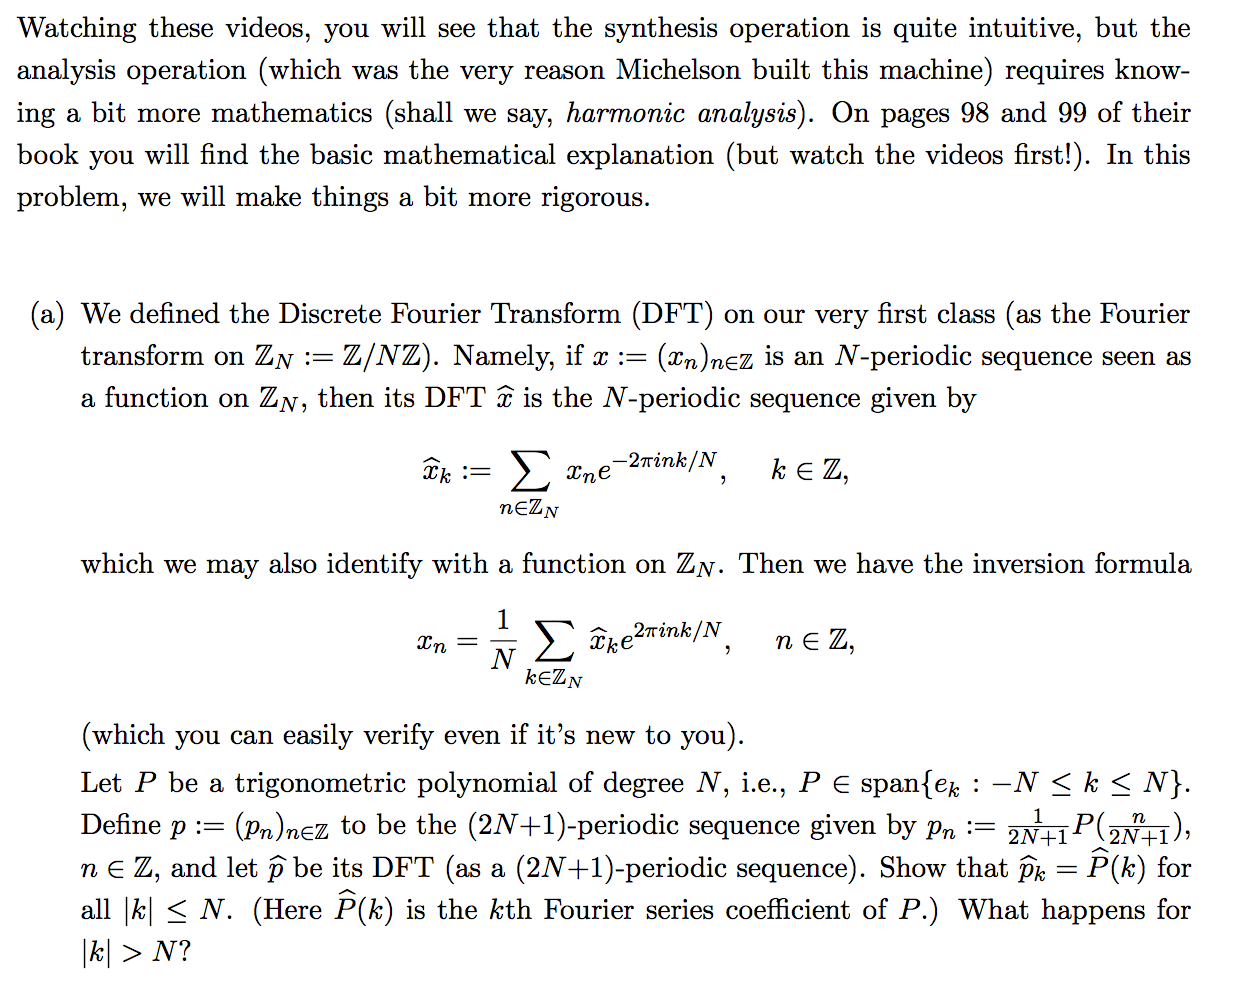
\includegraphics[width=0.8\textwidth]{HA-f-1.png}
\end{figure}
\end{question}

\newpage 

\begin{solution} \hfill \\
\textbf{(a)} Let $P$ be a trig polynomial defined on $\mathbb{T}$ of degree $N$, i.e. 
\eQb
P &=& \sum_{|k| \leq N} a_k e_k,
\eQe 
where $a_k$s are the complex coefficients. 
Suppose $|k| \leq N$. We trivially know that $\hat{P}(k) = a_k$. We compute the LHS as 
\eQb
\widehat{p_k} &=& \sum_{n \in \mathbb{Z}_{2N+1}} p_n e^{\frac{-2\pi i n k}{2N+1}} 
= \sum_{n \in \mathbb{Z}_{2N+1}} \dfrac{1}{2N+1} P(\dfrac{n}{2N + 1}) e^{-\frac{2\pi i n k}{2N+1}} \\
&=& \dfrac{1}{2N+1}\sum_{n \in \mathbb{Z}_{2N+1}} \left( 
\sum_{|l| \leq N} a_l e_{l}(\dfrac{n}{2N+1}) \right) 
e^{-\frac{2\pi i n k}{2N+1}} \\ 
&=& \dfrac{1}{2N+1}\sum_{n \in \mathbb{Z}_{2N+1}} \left( 
\sum_{|l| \leq N} a_l e^{\frac{2\pi i l n}{2N+1}} \right) 
e^{-\frac{2\pi i n k}{2N+1}} \\
&=& \dfrac{1}{2N+1}\sum_{n \in \mathbb{Z}_{2N+1}} \left( 
\sum_{|l| \leq N} a_l e^{\frac{2\pi i (l-k) n}{2N+1}} \right) 
= \dfrac{1}{2N+1}\sum_{n \in \mathbb{Z}_{2N+1}} a_n = a_n  
\eQe
as required. Now, for $|k| > N$, we see that $\widehat{p}_k = 0$, and $\hat{P}(k) = 0$ as well.

\end{solution}

\newpage

\begin{question}[1-2]
\hfill
\begin{figure}[h!]
  \centering
    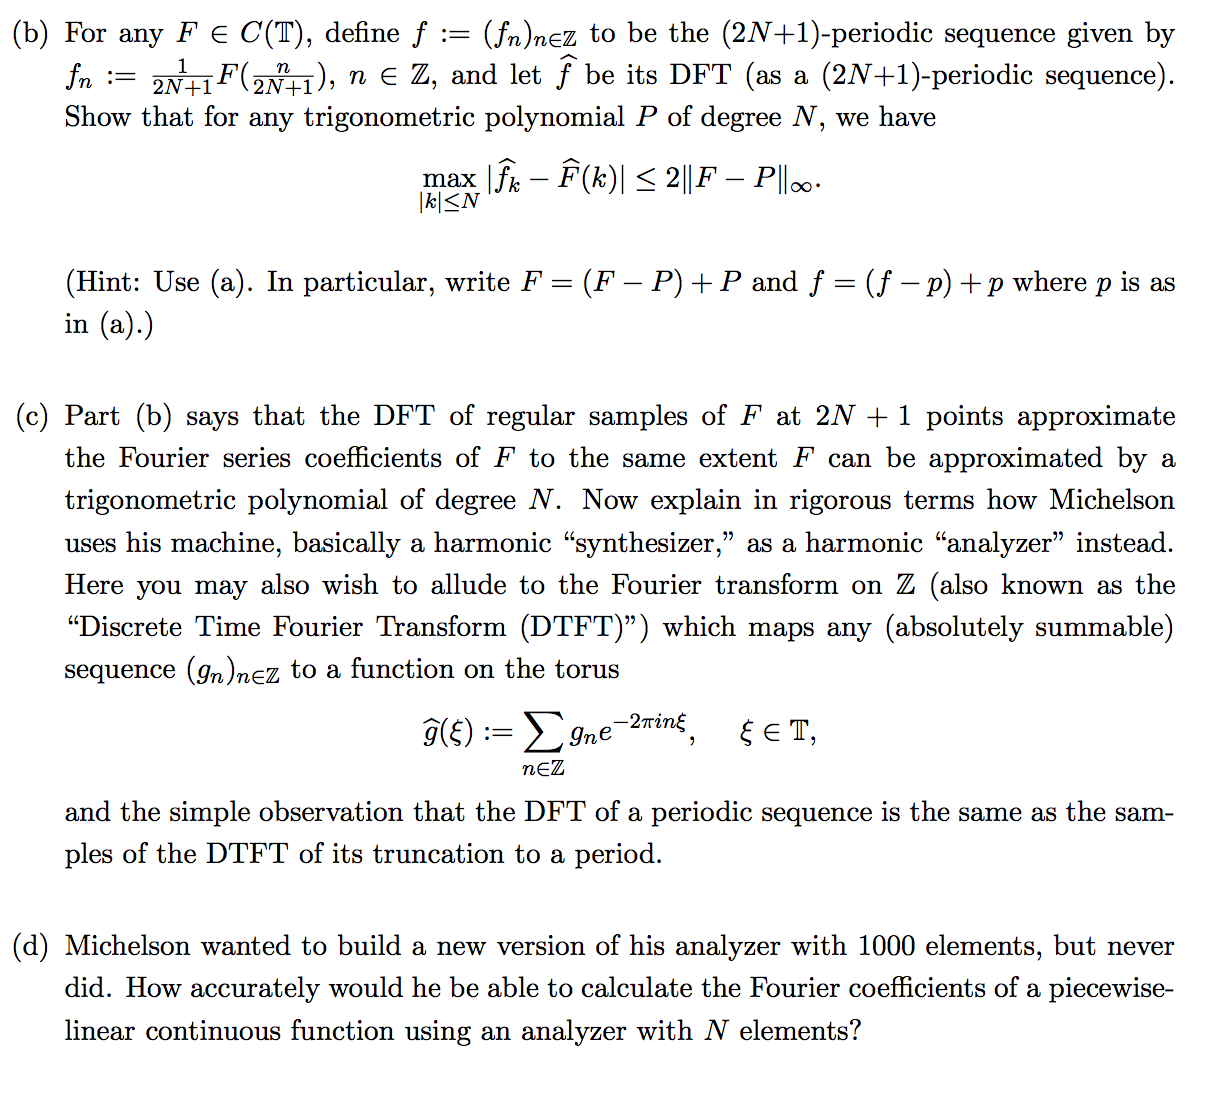
\includegraphics[width=0.8\textwidth]{HA-f-1-2.png}
\end{figure}
\end{question}
\begin{solution} \hfill \\
\textbf{(b)} Let $ f \in C(\mathbb{T})$, and $P$ be a trig polynomial of degree $N$. 
Define as before $f \triangleq (f_n)_{n \in \mathbb{Z}}$ to be the $(2N+1)$-periodic sequence given by 
\eQb
f_n \triangleq \dfrac{1}{2N+1}F(\dfrac{n}{2N+1}).
\eQe
With $F = (F- P) + P$ and $f = (f-p) + p$, by the result of $(a)$, for any $|k| \leq N$, we see that
\eQb
|\widehat{f_k} - \hat{F}_k| &=& |\reallywidehat{\{(f-p) + p\}}_k - 
\reallywidehat{(F-P)+P}(k)| \\ 
&=& |\widehat{(f-p)}_k - \reallywidehat{(F-P)}(k) + \hat{p}_k - \hat{P}(k)| \\
&\leq&  
|\widehat{(f-p)}_k| + |\reallywidehat{(F-P)}(k)| + | \hat{p}_k - \hat{P}(k)|. \\
&=&
|\widehat{(f-p)}_k| + |\reallywidehat{(F-P)}(k)|.
\eQe
Hence, as $N$ is finite, it suffices to show that for any $|k| \leq N$,
\eQb
|\widehat{(f-p)}_k| \leq ||F-P||_{\infty} \> \text{and} \> |\reallywidehat{(F-P)}(k)| \leq ||F-P||_{\infty}.
\eQe
Now, for $|k| \leq N$, the first inequality follows, as
\eQb
|\widehat{(f-p)}_k| &=& |\sum_{n \in \mathbb{Z}_{2N+1}} (f-p)_{n} e^{\frac{-2\pi i n k}{2N+1}}| \\
&=& |\dfrac{1}{2N+1} \sum_{n \in \mathbb{Z}_{2N+1}} (F(\dfrac{n}{2N+1}) - P(\dfrac{n}{2N+1}) )
e^{\frac{-2\pi i n k}{2N+1}}| \\
&\leq& \dfrac{1}{2N+1} \sum_{n \in \mathbb{Z}_{2N+1}} |F(\dfrac{n}{2N+1}) - P(\dfrac{n}{2N+1})| = ||F-P||_{\infty}.  
\eQe

\newpage

Likewise, for $|k| \leq N$, the second inequality, as $F-P \in C(\mathbb{T})$, and 
\eQb
|\reallywidehat{F-P}(k)| &=& \left| \int_{\mathbb{T}} (F-P)(t)e^{-ikt} dt \right|  \leq 
\int_{\mathbb{T}} |(F-P)(t)| dt \\
&=& ||F-P||_{1} \leq ||F-P||_{\infty}.
\eQe
Therefore, we have that for any trig polynomial of degree $N$, $P$, 
\eQb
\max_{|k| \leq N} | \hat{f}_{k} - \hat{F}(k)| &\leq& 2||F- P||_{\infty},
\eQe
as required. 


\end{solution}

\newpage

\begin{question}[2]
\hfill
\begin{figure}[h!]
  \centering
    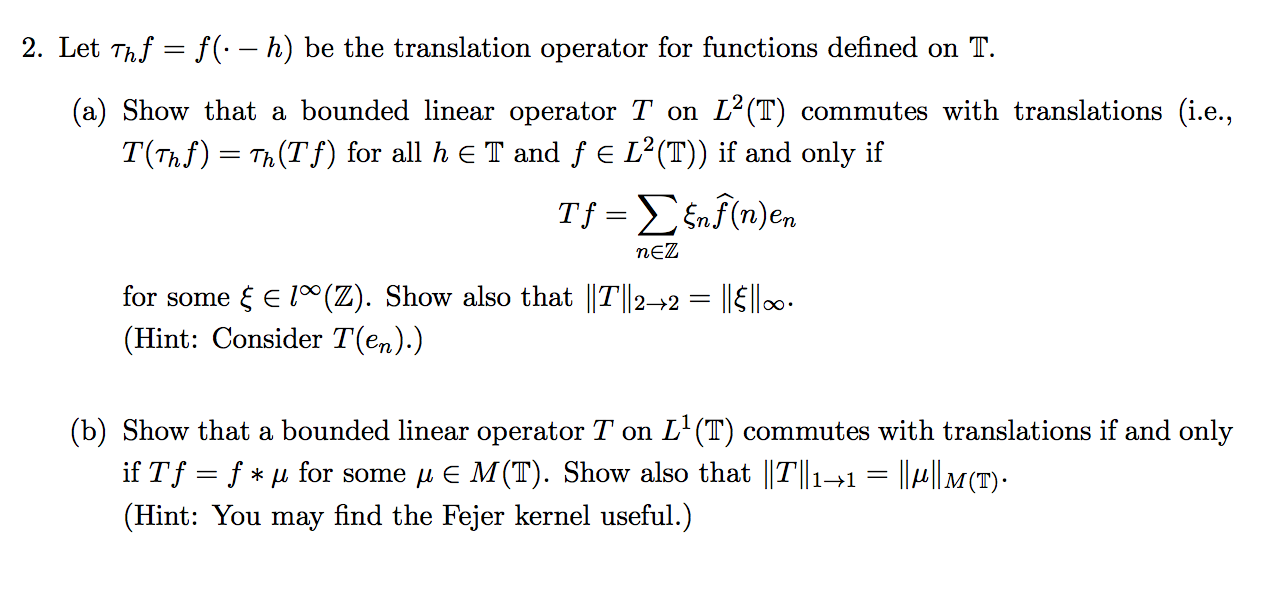
\includegraphics[width=0.8\textwidth]{HA-f-2.png}
\end{figure}
\end{question}
\begin{solution} \hfill \\
\textbf{(a)}
Fix $ h \in \mathbb{T}$. Suppose that, for some $\xi \in l^{\infty}(\mathbb{Z})$, we have
\eQb
Tf &=& \sum_{n \in \mathbb{Z}} \xi_{n} \hat{f}(n) e_n, 
\eQe
for some $\xi \in l^{\infty}(\mathbb{Z})$. It follows that, for any $n \in \mathbb{Z}$, by linearity of $T$,
\eQb
T(\tau_{h}(e_n)) &=& e^{-2\pi i n h} T(e_n) 
= e^{-2\pi i n h} \xi_n e_n = \tau_h(T(e_n)).
\eQe
With the fact that the trig polynomials are dense in $L^2$, through a standard density argument, we obtain
\eQb
T(\tau_{h}(f) &=& \tau_{h}(T(f)),
\eQe
as required. 
Conversely, 

Now, let $f = \dfrac{||\xi||_{\infty}}{|\xi_n|} e_n$ for some fixed $n$. By the established equivalence, 
it follows that 
\eQb
||Tf||_{2} &=& 
\eQe

\bigskip

\textbf{(b)} Consider the Fejer kernel, denoted by $\{ K_n \}$. 
Firstly, observe that as the Fejer kernel is an approximate identity,
we have $\sup_{N} \int_{0}^{1} |K_n(x)|dx < \infty$, so 
we can extract a subsequence $\{ K_{n_l} \}$ 
such that $K_{n_l} \to \mu$ weakly in $L^1$, for some $\mu \in M(\mathbb{T})$.
 For notational convenience, we
relabel the subsequence as $\{ K_n \}$. Now, assume that $T$ commutes 
with translations. It follows that, for any $f \in C(\mathbb{T})$, and $x \in \mathbb{T}$, 
\eQb
f * \mu (x) &=& \lim_{n \to \infty} \int_{\mathbb{T}} f(t)T(K_n) (x - t) dt 
= \lim_{n \to \infty} \int_{\mathbb{T}} f(t)T(K_n(x - t)) dt, \\
&=& \lim_{n \to \infty} \int_{\mathbb{T}} T(f(t)(K_n) (x - t)) dt, 
= \lim_{n \to \infty} T\left(\int_{\mathbb{T}} f(t) K_n(x-t) dt \right),
\eQe
which via boundedness of $T$ and the fact that $f \in C(\mathbb{T})$, 
\eQb
\lim_{n \to \infty} (f*K_n) (x) = f(x),
\eQe
implies that
\eQb
f* \mu(x)&=& T \left( \lim_{n \to \infty} \int_{\mathbb{T}} f(t) K_n(x-t) dt \right) = Tf(x),
\eQe  
as required. Now, as $C(\mathbb{T})$ is dense in $L^1(\mathbb{T})$, it follows that
\eQb
f* \mu &=& Tf 
\eQe 


\end{solution}

\newpage

\begin{question}[3]
\hfill
\begin{figure}[h!]
  \centering
    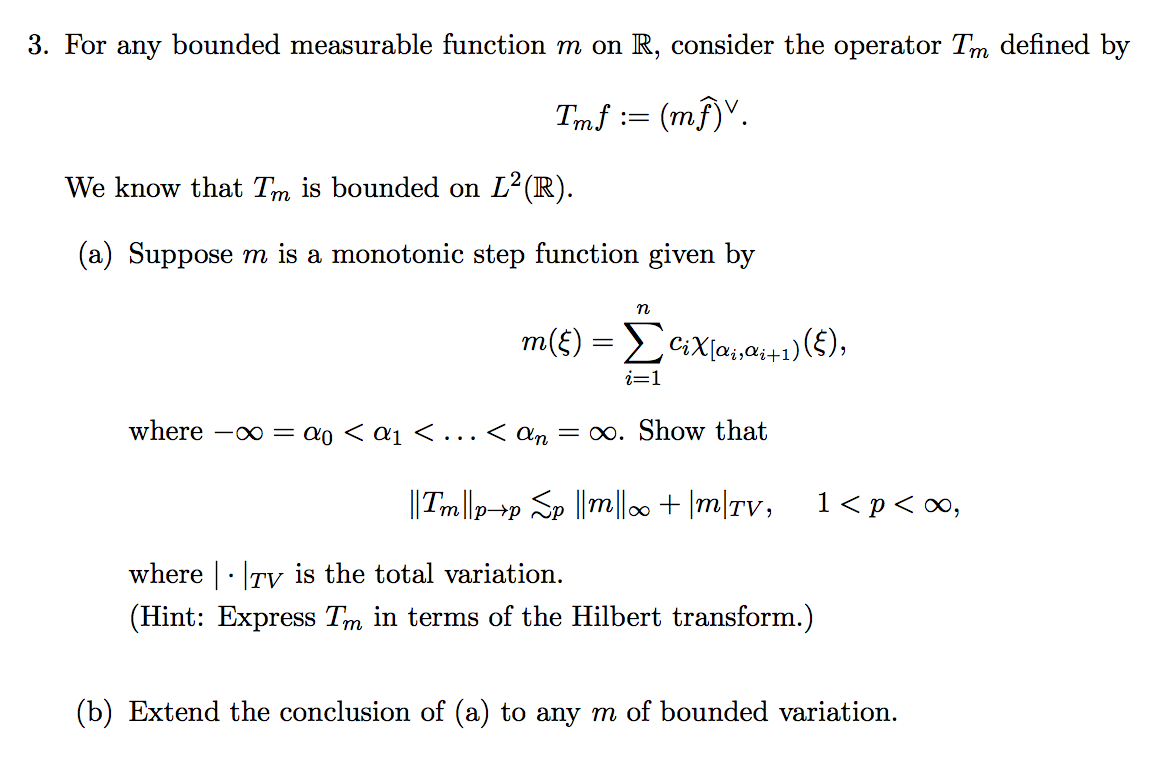
\includegraphics[width=0.8\textwidth]{HA-f-3.png}
\end{figure}
\end{question}
\begin{solution} \hfill \\
\textbf{(a)} Suppose $m$ is a monotonic step function given by 
\eQb
T_{m}f &=& (m\hat{f})^{\wedge} = \left( \sum_{i=1}^{n} c_i X_{[\alpha_{i}, \alpha_{i+1})} \hat{f}\right)^{\wedge}.
\eQe
Under this setting, we simply have that 
\eQb
||m||_{\infty} = \max_{i}| |c_i| \> \text{ and } \> |m|_{TV} = \sum_{i=1}^{n-1} |c_{i+1} - c_{i}|  
\eQe
We have that
\eQb
||T_m||_{p \to p} \leq  C(p) 
\eQe



\bigskip

\textbf{(b)}
\end{solution}

\newpage

\begin{question}[4]
\hfill
\begin{figure}[h!]
  \centering
    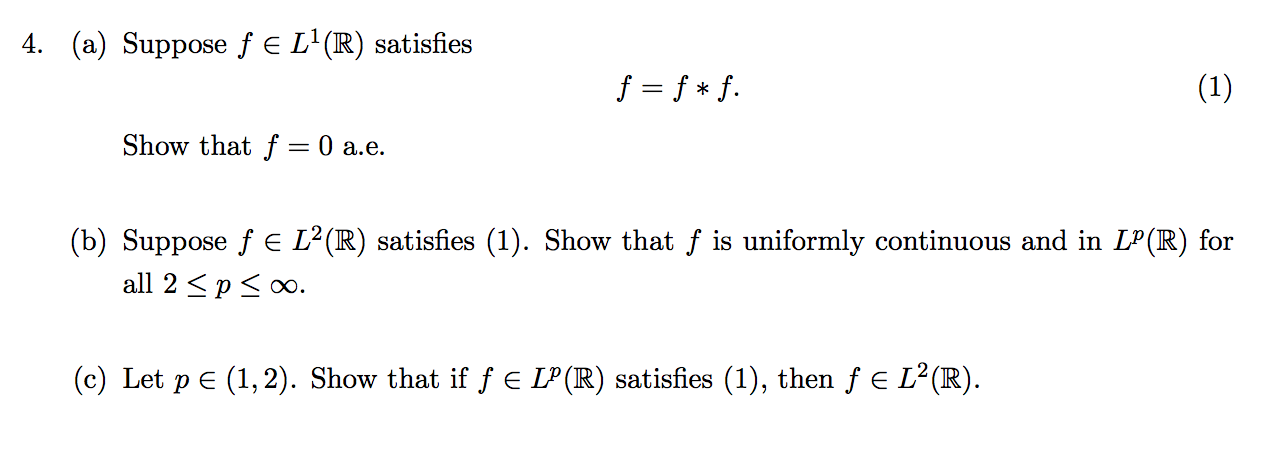
\includegraphics[width=0.8\textwidth]{HA-f-4.png}
\end{figure}
\end{question}
\begin{solution} \hfill \\

\textbf{(a)} Let $f \in L^1$. Taking the Fourier transform on both sides gives
\eQb
\hat{f} &=& \hat{f}\hat{f},
\eQe
which, with the continuity of $\hat{f}$, implies that
\eQb
\hat{f} = 0 \> \text{ a.e} \> &\text{ or }& \> \hat{f} = 1 \> \text{a.e}.
\eQe
As $\hat{f} = 1 \> \text{ a. e}$ contradicts the Riemann-Lebesgue lemma, it follows that
\eQb
\hat{f} &=& 0 \> \text{ a.e.},
\eQe
so by the inversion formula for $L^1$
\eQb
f &=& 0 \> \text{ a.e.},
\eQe 
as required.

\bigskip

\textbf{(b)} Let $f \in L^2$ such that $f = f * f$. By the same argument in the $L^1$ case, 
we have 
\eQb
\hat{f} = 0 \> \text{ a.e} \> &\text{ or }& \> \hat{f} = 1 \> \text{a.e}.
\eQe
Let $E_1 = \{ \hat{f} = 1\}$ and $E_0 = \{ \hat{f} = 0 \}$. Note that
as $\hat{f} \in L^2$, it follows that $m(E_1) < \infty$. Now, by the inversion formula for $L^2$,
we obtain
\eQb
f(x) &=& \int_{\mathbb{R}} \hat{f}(\xi)e^{2\pi i \xi x} d\xi = \int_{E_1} e^{2\pi i \xi x} d\xi. 
\eQe
Now, for any $\delta > 0$ and $x \in \mathbb{R}$, it follows that
\eQb
|f(x + \delta) - f(x)| &=& | \int_{E_1} e^{2\pi i \xi (x + \delta)}  - 
e^{2\pi i \xi x}| d\xi  
\leq  \int_{E_1} |e^{2\pi i \xi x }| |e^{2\pi i \xi \delta } - 1| d\xi \\
&\leq& 
\int_{E_1} |e^{2\pi i \xi \delta } - 1| d\xi. \\
\eQe
Observe that the last integral is independent of $x$, and the integrand tends to $0$,
as $\delta \to 0$. Therefore, we have shown that $f$ is uniformly continuous. We now argue that
$f \in L^p$ for $p \in [2,\infty]$. Fix $p \in [2,\infty]$.  


\bigskip

\textbf{(c)} 

\end{solution}
\end{document}
